\chapter{Lec 14 - Practical Methodology}

\section{Practical Methodology}
During day to day development of machine learning systems, practitioners need to decide whether to gather more data, increase or decrease model capacity, add or remove regularizing features, improve the optimization of a model, improve approximate inference in a model, or debug the software implementation of the model.\newline\newline
We recommend the following practical design process:
\begin{itemize}
    \item Determine your goals—what error metric to use, and your target value for
    this error metric. These goals and error metrics should be driven by the
    problem that the application is intended to solve.

    \item Establish a working end-to-end pipeline as soon as possible, including the estimation of the appropriate performance metrics.

    \item Instrument the system well to determine bottlenecks in performance. Diagnose which components are performing worse than expected and whether it is due to overfitting, underfitting, or a defect in the data or software.

    \item Repeatedly make incremental changes such as gathering new data, adjusting
    hyperparameters, or changing algorithms, based on specific findings from
    your instrumentation.
\end{itemize}


\subsection{Performance Metrics}
Keep in mind that for most applications, it is impossible to achieve absolute
zero error. The Bayes error defines the minimum error rate that you can hope to
achieve, even if you have infinite training data and can recover the true probability distribution. This is because your input features may not contain complete information about the output variable, or because the system might be intrinsically stochastic. You will also be limited by having a finite amount of training data.\newline\newline
An important aspect is the choice of which metric to use. Several different performance metrics may be used to measure the effectiveness of a complete application that includes machine learning components. It is common to measure the accuracy, or equivalently, the error rate, of a system. However, many applications require more advanced metrics. For example, for an e-mail spam detection system it is much worse to block a legitimate message than to allow a questionable message to pass through. Rather than measuring the error rate of a spam classifier, we may wish to measure some form of total cost, where the cost of blocking legitimate messages is higher than the cost of allowing spam messages.\newline\newline
Sometimes we wish to train a binary classifier that is intended to detect some rare event. Consider a disease that only one in 1M people have. We can easily achieve 99.9999\% accuracy on the detection task, by simply hard-coding the classifier to always report that the disease is absent. Clearly, accuracy is a poor way to characterize the performance of such a system. One way to solve this problem is to instead measure \textbf{precision} and \textbf{recall}. Before introducing these measures, let's define the contingency table:
\begin{center}
    \begin{tabular}{c|c|c}
         & Relevant & Not relevant  \\
         \hline
         Retrieved & True Positive (TP) & False Positive (FP) \\
         Not Retrieved & False Negative (FN) & True Negative (TN)
    \end{tabular}
\end{center}
The accuracy $\alpha$ is defined as follows:
\[\alpha = \frac{TP + TN}{TP + TN + FP + FN}\]
If relevance is assumed to be \textbf{binary-valued}, effectiveness is typically measured as a combination of:
\begin{itemize}
    \item \textbf{Precision}: 
    \[\pi = \frac{TP}{TP + FP}\]
    is the fraction of detections reported by the model that were correct.

    \item \textbf{Recall:}
    \[\rho = \frac{TP}{TP + FN}\]
    is the fraction of true events that were detected.
\end{itemize}
A detector that says no one has the disease would achieve
zero precision, and zero recall. A detector that says everyone has the disease would achieve perfect recall, but precision equal to the percentage of people who have the disease (0.0001\% in our example of a disease that only one people in a million have).\newline\newline
When using precision and recall, it is common to plot a \textbf{PR curve}, with precision on the y-axis and recall on the x-axis. The classifier generates a score
that is higher if the event to be detected occurred.
\newline\newline
In some cases, it may be necessary to get a trade-off between Precision and Recall. This can be done using the \textbf{F-measure}, which is a weighted harmonic mean of the Precision ($\pi$) and Recall ($\rho$):
\[F_{\beta} = \frac{(1 + \beta^{2})\pi \rho}{\beta^{2}\pi + \rho}\]
If $\beta < 1$ it emphasizes Precision, while $\beta > 1$ emphasizes Recall. When $\beta = 1$, we obtain the so called F1 score:
\[F_{1} = 2\frac{\pi\rho}{\pi + \rho}\]

\subsection{Coverage}
In some applications, it is possible for the machine learning system to refuse to make a decision. It is useful when a wrong decision can be harmful and/or if a human operator is able to occasionally take over. A natural performance metric to use in this situation is \textbf{coverage}. Coverage is the fraction of examples for which the machine learning system is able to produce a response. It is possible to trade coverage for accuracy. One can always obtain 100\% accuracy
by refusing to process any example, but this reduces the coverage to 0\%.

\subsection{Baseline models}
Baselines are simple models chosen to provide a first estimation of the achievable level of performance. Depending on the complexity of your problem, you may even want to begin without using deep learning. If your problem has a chance of being solved by just choosing a few linear weights correctly, you may want to begin with a simple statistical model like logistic regression.\newline\newline
First, choose the general category of model based on the structure of your data ( e.g. if you want to perform supervised learning with fixed-size vectors as input, use a feedforward network with fully connected layers). You should begin by using some kind of piecewise linear
unit (ReLUs or their generalizations like Leaky ReLUs, PreLus and maxout). If your input or output is a sequence, use a gated recurrent net (LSTM or GRU).\newline\newline
A reasonable choice of optimization algorithm is SGD with momentum with a decaying learning rate. Another very reasonable alternative is Adam.\newline\newline
While it is reasonable to omit batch normalization from the very first baseline, it should be introduced quickly if optimization appears to be problematic.\newline\newline
Unless your training set contains tens of millions of examples or more, you should include some mild forms of regularization from the start (e.g. early stopping, dropout, etc.).\newline\newline
A common question is whether to begin by using unsupervised learning. This is somewhat domain specific. Some domains, such
as natural language processing, are known to benefit tremendously from unsuper- vised learning techniques such as learning unsupervised word embeddings. In other domains, such as computer vision, current unsupervised learning techniques do not bring a benefit.

\subsection{Determine whether to gather more data}
After the first end-to-end system is established, it is time to measure the performance of the algorithm and determine how to improve it. Many machine learning novices are tempted to make improvements by trying out many different algorithms. However, it is often much better to gather more data than to improve the learning algorithm.\newline\newline
First, determine whether the performance on the training set is acceptable. If performance on the training set is poor, the learning algorithm is not using the training data that is already
available, so there is no reason to gather more data. Instead, try increasing the size of the model by adding more layers or adding more hidden units to each layer.\newline\newline
Also, try improving the learning algorithm, for example by tuning the learning rate hyperparameter. If large models and carefully tuned optimization algorithms do not work well, then the problem might be the quality of the training data. The data may be too noisy or may not include the right inputs needed to predict the desired outputs. This suggests starting over, collecting cleaner data or collecting a richer set of features.\newline\newline
If test set performance is much worse than training set performance, then gathering more data is one of the most effective solutions.
If gathering much more data is not feasible, the only other way to improve generalization error is to improve the learning algorithm itself. This becomes the domain of research and not the domain of advice for applied practitioners.

\subsection{Selecting Hyperparameters}
Most deep learning algorithms come with many hyperparameters that control many aspects of the algorithm’s behavior. There are two basic approaches to choosing these hyperparameters: choosing them manually and choosing them automatically.\newline\newline
The primary goal of \textbf{manual hyperparameter} search is to adjust the effective capacity of the model to match the complexity of the task.
\newline\newline
The generalization error typically follows a U-shaped curve
\begin{center}
    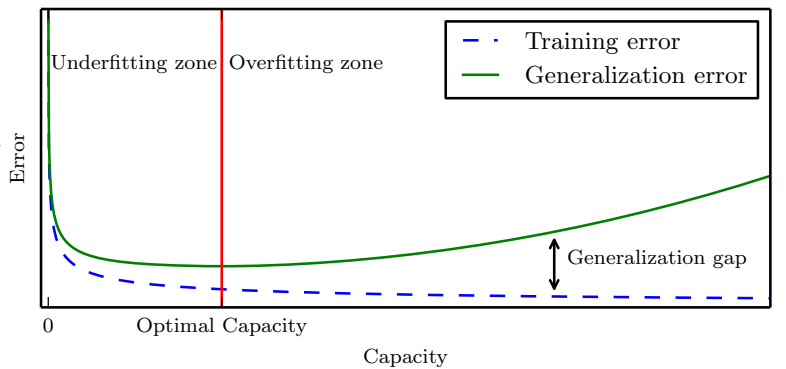
\includegraphics[]{images/Gen-error.png}
\end{center}
At one extreme, the hyperparameter value corresponds to low capacity, and generalization error is high because training error is high. This is the underfitting regime. At the other extreme, the hyperparameter value corresponds to high capacity, and the generalization error is high because the gap between training and test error is high. Somewhere in the middle lies the optimal model capacity, which achieves the lowest possible generalization error, by adding a medium generalization gap to a medium amount of training error.\newline\newline
The learning rate is perhaps the most important hyperparameter. The effective capacity of the model is highest when the learning rate is correct for the optimization problem, not when the learning rate is especially large or especially small. The learning rate has a U-shaped curve for training error.
\begin{center}
    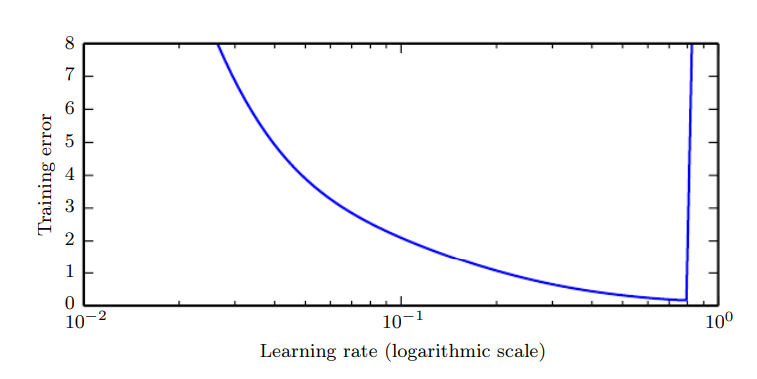
\includegraphics[]{images/lr.png}
\end{center}
Tuning the parameters other than the learning rate requires monitoring both
training and test error to diagnose whether your model is overfitting or underfitting, then adjusting its capacity appropriately.\newline\newline
Manual hyperparameter tuning can work very well when the user has a good starting point, such as one determined by others having worked on the same type of application and architecture. However, for many applications, these starting points are not available. In these cases, \textbf{automated algorithms} can find useful values of the hyperparameters. It is possible, in principle, to develop hyperparameter optimization algorithms that wrap a learning algorithm and choose its hyperparameters. Unfortunately, hyperparameter optimization algorithms often have their own hyperparameters, such as the range of values that
should be explored for each of the learning algorithm’s hyperparameters.\newline\newline
When there are three or fewer hyperparameters, the common practice is to perform \textbf{grid search}. For each hyperparameter, the user selects a small finite set of values to explore. The grid search algorithm then trains a model for every joint specification of hyperparameter values in the Cartesian product of the set of values for each individual hyperparameter. The experiment that yields the best validation set error is then chosen as having found the best hyperparameters. The obvious problem with grid search is that its computational cost grows
exponentially with the number of hyperparameters.\newline\newline
Fortunately, there is an alternative to grid search that is as simple to program, more convenient to use, and converges much faster to good values of the hyperparameters: \textbf{random search}\newline\newline
Lastly, there are other approaches for tuning hyperparameters, e.g.,  \textbf{model-based} (Bayesian). In this case the search for good hyperparameters is cast as an optimization problem. The decision variables are the hyperparameters. The cost to be optimized is the validation set error that results from training using these hyperparameters.

\subsection{Debugging Strategies}
Machine learning systems are difficult to debug for a variety of reasons. Some important debugging tests include:
\begin{itemize}
    \item Visualize the model in action.
    \item Visualize the worst mistakes.
    \item Fit a tiny dataset: If you have high error on the training set, determine whether it is due to genuine underfitting or due to a software defect.
    \item Check the gradient (exploding or vanishing).
    \item Check the activations: how many neurons fire? ReLU can induce “dead” neurons.
\end{itemize}

